\documentclass[11pt]{article}

% ---------- Packages ----------
\usepackage[margin=0.75in]{geometry}
\usepackage{amsmath,amssymb,amsfonts}
\usepackage{mathtools}
\usepackage{array,booktabs,tabularx,multicol}
\usepackage{graphicx}
\usepackage{tikz,pgfplots}
\usepackage{tcolorbox}
\usepackage{xcolor}
\usepackage{enumitem}
\usepackage{fancyhdr}
\usepackage{lastpage}
\usepackage{needspace}

\pgfplotsset{compat=1.18}
\usetikzlibrary{arrows.meta,calc,angles,quotes,patterns}

% =========================
% Novel Prep Brand Colors
% =========================
\definecolor{nppurple}{RGB}{98,54,255}
\definecolor{nppurple2}{RGB}{76,42,204}
\definecolor{nplight}{RGB}{240,235,255}
\definecolor{npsoft}{RGB}{248,246,255}
\definecolor{npgray}{RGB}{226,222,238}

% ---------- Header/Footer ----------
\pagestyle{fancy}
\fancyhf{}
\lhead{\textcolor{nppurple2}{\textbf{Novel Prep Learning Center}}}
\rhead{\textcolor{nppurple2}{\textbf{Math I / Enhanced Math I Placement}}}
\cfoot{\textcolor{nppurple2}{\thepage\ of \pageref{LastPage}}}
\setlength{\headheight}{14pt}
\renewcommand{\headrulewidth}{0.4pt}
\renewcommand{\footrulewidth}{0pt}

% ---------- Boxes ----------
\newtcolorbox{titlebox}{
colback=nplight,
colframe=nppurple2,
boxrule=0.95pt,
arc=2pt,
left=8pt,
right=8pt,
top=8pt,
bottom=8pt
}

\newtcolorbox{problemBox}{
colback=white,
colframe=npgray,
boxrule=0.7pt,
arc=2pt,
left=8pt,
right=8pt,
top=8pt,
bottom=8pt
}

\newtcolorbox{scoreCard}{
colback=npsoft,
colframe=npgray,
boxrule=0.7pt,
arc=2pt,
left=8pt,
right=8pt,
top=8pt,
bottom=8pt
}

\newtcolorbox{sectionNote}{
colback=white,
colframe=nppurple2,
boxrule=0.75pt,
arc=2pt,
left=8pt,
right=8pt,
top=7pt,
bottom=7pt
}

\newtcolorbox{partBox}{
colback=nplight,
colframe=nppurple2,
boxrule=0.85pt,
arc=2pt,
left=8pt,
right=8pt,
top=6pt,
bottom=6pt
}

\newtcolorbox{solutionBox}{
colback=npsoft,
colframe=nppurple2,
title=\textbf{Step-by-Step Solution},
boxrule=0.8pt,
arc=2pt,
left=8pt,
right=8pt,
top=8pt,
bottom=8pt
}

\setlength{\parindent}{0pt}
\setlength{\parskip}{0.35em}
\renewcommand{\arraystretch}{1.18}
\setlist[enumerate,1]{itemsep=0.75em,topsep=0.4em,label=\protect\circnum{\arabic*},leftmargin=*}
\setlist[enumerate,2]{itemsep=0.2em,topsep=0.2em}
\newcolumntype{L}[1]{>{\raggedright\arraybackslash}m{#1}}

% ---------- Commands ----------
\newcommand{\circnum}[1]{%
\begin{tikzpicture}[baseline=(char.base)]
\node[
draw=nppurple2,
circle,
inner sep=1.4pt,
line width=0.9pt,
text=nppurple2
] (char) {\strut\small #1};
\end{tikzpicture}}

\newcommand{\ansline}{\rule{2.5in}{0.4pt}}
\newcommand{\pts}[1]{\hfill\textbf{[#1 pts]}}
\newcommand{\spacefor}[1]{\vspace*{#1}}
\newcommand{\blankline}[1]{\rule{#1}{0.4pt}}
\newcommand{\work}{\vspace{1.8cm}}
\newcommand{\longwork}{\vspace{4.2cm}}
\newcommand{\choices}[4]{
\begin{multicols}{4}
\begin{enumerate}[label=\Alph*.]
\item #1
\item #2
\item #3
\item #4
\end{enumerate}
\end{multicols}
}

\newcommand{\question}[5]{
\item #1
\choices{#2}{#3}{#4}{#5}
\vspace{0.6em}
}

\newcommand{\grid}{
\begin{center}
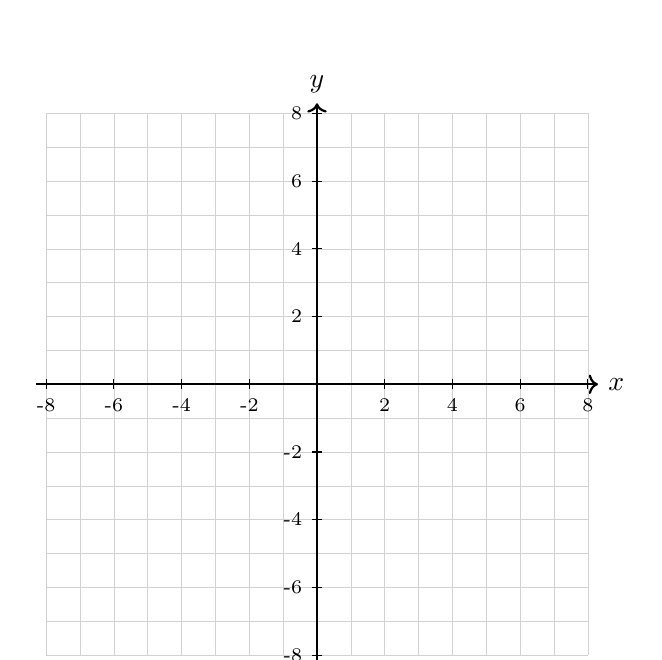
\begin{tikzpicture}[scale=0.43]
\draw[step=1cm,gray!35,very thin] (-8,-8) grid (8,8);
\draw[->,thick] (-8.3,0)--(8.3,0) node[right] {$x$};
\draw[->,thick] (0,-8.3)--(0,8.3) node[above] {$y$};
\foreach \x in {-8,-6,-4,-2,2,4,6,8} \draw (\x,0.15)--(\x,-0.15) node[below] {\scriptsize \x};
\foreach \y in {-8,-6,-4,-2,2,4,6,8} \draw (0.15,\y)--(-0.15,\y) node[left] {\scriptsize \y};
\end{tikzpicture}
\end{center}
}

\begin{document}

\begin{center}
    {\LARGE \textbf{Novel Prep Learning Center}}\\[0.2em]
    {\Large \textbf{Math I / Enhanced Math I Placement Exam}}\\[0.25em]
    {\large IUSD-Aligned Readiness Diagnostic}\\[0.6em]
    Name:\ \ansline \hfill Date:\ \ansline
\end{center}

\begin{titlebox}
\textbf{Directions:} Read each question carefully. Choose the best answer for multiple-choice questions. Show all work for graphing and free-response questions. Simplify all final answers.
\end{titlebox}

\begin{problemBox}
\textbf{Teacher Use:} This diagnostic is designed to answer two placement questions. First, is the student ready for Math I? Second, if Math I readiness is secure, is the student ready for Enhanced Math I? Part A checks core algebra. Part B measures Math I outcomes. Part C and the extended free-response tasks emphasize Enhanced Math I readiness signals: radicals, Pythagorean reasoning, stronger modeling, systems, transformations, coordinate geometry, and proof.
\end{problemBox}

\vspace{0.1in}
\begin{scoreCard}
\renewcommand{\arraystretch}{1.25}
\begin{tabularx}{\textwidth}{>{\bfseries\color{nppurple2}}L{2.6cm}X}
Purpose & Gate 1 confirms Math I readiness; Gate 2 confirms Enhanced Math I readiness after Gate 1 is secure.\\
Structure & 50 multiple-choice questions, graphing, free response, scoring guide, study plan, and answer key.\\
Use & Placement decisions should prioritize the two diagnostic gates.
\end{tabularx}
\end{scoreCard}

\newpage
\section*{Multiple Choice Questions}
\begin{sectionNote}
Questions 1-30 are used primarily for Math I readiness. Questions 31-50 add Enhanced Math I readiness signals.
\end{sectionNote}
\begin{partBox}
{\large \textcolor{nppurple2}{\textbf{Part A --- Core Readiness}}}
\end{partBox}
\begin{enumerate}
\item Solve for $x$: $-3x+7=25$.
\begin{enumerate}[label=(\Alph*)]
\item $x=-6$ \item $x=6$ \item $x=-\frac{32}{3}$ \item $x=\frac{32}{3}$
\end{enumerate}

\item Which expression is equivalent to $4(2x-5)-3(x+1)$?
\begin{enumerate}[label=(\Alph*)]
\item $5x-23$ \item $11x-17$ \item $5x-17$ \item $8x-8$
\end{enumerate}

\item Solve: $\frac{2x-5}{3}=7$.
\begin{enumerate}[label=(\Alph*)]
\item $x=8$ \item $x=11$ \item $x=13$ \item $x=26$
\end{enumerate}

\item Which inequality represents the solution to $-4x+9<21$?
\begin{enumerate}[label=(\Alph*)]
\item $x<-3$ \item $x>-3$ \item $x<3$ \item $x>3$
\end{enumerate}

\item Which relation is a function?
\begin{enumerate}[label=(\Alph*)]
\item $\{(1,2),(1,4),(3,6)\}$ \item $\{(-2,5),(0,5),(2,5)\}$
\item $\{(3,1),(3,2),(3,3)\}$ \item $\{(0,0),(0,1),(1,0)\}$
\end{enumerate}

\Needspace{7\baselineskip}
\item The slope of the line through $(-2,5)$ and $(4,-7)$ is:
\begin{enumerate}[label=(\Alph*)]
\item $2$ \item $-2$ \item $\frac{1}{2}$ \item $-\frac{1}{2}$
\end{enumerate}

\item What is the $y$-intercept of $3x-2y=10$?
\begin{enumerate}[label=(\Alph*)]
\item $(0,-5)$ \item $(0,5)$ \item $(\frac{10}{3},0)$ \item $(-5,0)$
\end{enumerate}

\item Which equation has infinitely many solutions?
\begin{enumerate}[label=(\Alph*)]
\item $2(x+3)=2x+5$ \item $3x-4=2x+8$ \item $5(x-1)=5x-5$ \item $4x+1=4x-1$
\end{enumerate}

\item Simplify $\sqrt{72}$.
\begin{enumerate}[label=(\Alph*)]
\item $6\sqrt{2}$ \item $12\sqrt{6}$ \item $8\sqrt{9}$ \item $36\sqrt{2}$
\end{enumerate}

\item If $f(x)=2x^2-3x+1$, what is $f(-2)$?
\begin{enumerate}[label=(\Alph*)]
\item $3$ \item $9$ \item $15$ \item $-1$
\end{enumerate}

\newpage
\begin{partBox}
{\large \textcolor{nppurple2}{\textbf{Part B --- Math I Mastery}}}
\end{partBox}
\item Which table represents an exponential function?
\begin{multicols}{2}
\begin{enumerate}[label=(\Alph*)]
\item $\begin{array}{c|cccc}x&0&1&2&3\\ \hline y&3&6&9&12\end{array}$
\item $\begin{array}{c|cccc}x&0&1&2&3\\ \hline y&5&10&20&40\end{array}$
\item $\begin{array}{c|cccc}x&0&1&2&3\\ \hline y&2&5&10&17\end{array}$
\item $\begin{array}{c|cccc}x&0&1&2&3\\ \hline y&9&7&5&3\end{array}$
\end{enumerate}
\end{multicols}

\item The function $g(x)=120(0.85)^x$ models a phone battery after $x$ hours. Which statement is true?
\begin{enumerate}[label=(\Alph*)]
\item The initial battery level is $85\%$ and it grows by $120\%$ each hour.
\item The initial battery level is $120$ and it decreases by $15\%$ each hour.
\item The initial battery level is $120$ and it decreases by $85\%$ each hour.
\item The initial battery level is $0.85$ and it grows by $20\%$ each hour.
\end{enumerate}

\item A line is perpendicular to $y=\frac{4}{5}x-2$ and passes through $(8,1)$. Which equation represents the line?
\begin{enumerate}[label=(\Alph*)]
\item $y=-\frac{5}{4}x+11$ \item $y=\frac{4}{5}x-\frac{27}{5}$
\item $y=-\frac{4}{5}x+\frac{37}{5}$ \item $y=\frac{5}{4}x-9$
\end{enumerate}

\item Which system has the solution $(2,-1)$?
\begin{enumerate}[label=(\Alph*)]
\item $\begin{cases}x+y=3\\2x-y=5\end{cases}$ \item $\begin{cases}x-y=3\\3x+y=6\end{cases}$
\item $\begin{cases}2x+y=3\\x+2y=1\end{cases}$ \item $\begin{cases}x+2y=0\\4x-y=9\end{cases}$
\end{enumerate}

\item Solve the system: $\begin{cases}2x+y=11\\x-y=1\end{cases}$.
\begin{enumerate}[label=(\Alph*)]
\item $(3,5)$ \item $(4,3)$ \item $(5,1)$ \item $(2,7)$
\end{enumerate}

\item A gym charges a sign-up fee plus a monthly fee. The cost is \$95 after 2 months and \$185 after 5 months. What is the monthly fee?
\begin{enumerate}[label=(\Alph*)]
\item \$20 \item \$25 \item \$30 \item \$45
\end{enumerate}

\item The first term of an arithmetic sequence is $-7$ and the common difference is $5$. Which formula gives the $n$th term?
\begin{enumerate}[label=(\Alph*)]
\item $a_n=-7+5n$ \item $a_n=-7+5(n-1)$ \item $a_n=5(-7)^{n-1}$ \item $a_n=-7(5)^{n-1}$
\end{enumerate}

\item The first term of a geometric sequence is $6$ and the common ratio is $\frac{1}{3}$. What is the fifth term?
\begin{enumerate}[label=(\Alph*)]
\item $\frac{2}{9}$ \item $\frac{2}{27}$ \item $\frac{6}{27}$ \item $\frac{1}{162}$
\end{enumerate}

\item Which interval represents $x\geq -2$ and $x<5$?
\begin{enumerate}[label=(\Alph*)]
\item $(-2,5)$ \item $[-2,5)$ \item $(-2,5]$ \item $[-2,5]$
\end{enumerate}

\item The two-way table shows student activity choices.
\[
\begin{array}{|c|c|c|c|}
\hline
&\text{Art}&\text{Robotics}&\text{Total}\\ \hline
\text{Grade 9}&18&27&45\\ \hline
\text{Grade 10}&22&13&35\\ \hline
\text{Total}&40&40&80\\ \hline
\end{array}
\]
What percentage of Grade 9 students chose Robotics?
\begin{enumerate}[label=(\Alph*)]
\item $27\%$ \item $33.75\%$ \item $60\%$ \item $67.5\%$
\end{enumerate}

\newpage
\item A data set is $\{4,6,7,8,10,12,25\}$. Which statement is true?
\begin{enumerate}[label=(\Alph*)]
\item The mean is less than the median because $25$ is an outlier.
\item The mean is greater than the median because $25$ is an outlier.
\item The mean equals the median.
\item The range is $12$.
\end{enumerate}

\item The box plot below represents a data set. What is the interquartile range?
\begin{center}
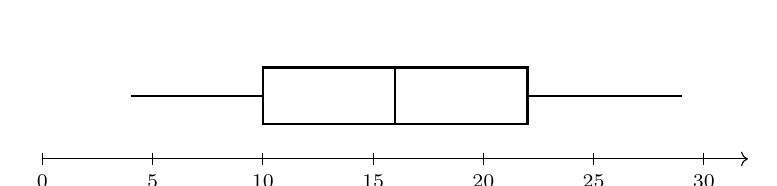
\begin{tikzpicture}[xscale=0.28,yscale=0.8]
\draw[->] (0,0)--(32,0);
\foreach \x in {0,5,10,15,20,25,30} \draw (\x,0.1)--(\x,-0.1) node[below] {\scriptsize \x};
\draw[thick] (4,1)--(10,1);
\draw[thick] (22,1)--(29,1);
\draw[thick] (10,0.55) rectangle (22,1.45);
\draw[thick] (16,0.55)--(16,1.45);
\end{tikzpicture}
\end{center}
\begin{enumerate}[label=(\Alph*)]
\item $6$ \item $12$ \item $18$ \item $25$
\end{enumerate}

\item A scatter plot has a line of best fit $y=4.8x+12.5$. Which is the best prediction when $x=9$?
\begin{enumerate}[label=(\Alph*)]
\item $43.2$ \item $55.7$ \item $108$ \item $17.3$
\end{enumerate}

\item Triangle $ABC$ has vertices $A(1,2)$, $B(5,2)$, and $C(1,7)$. What is the length of $\overline{BC}$?
\begin{enumerate}[label=(\Alph*)]
\item $3$ \item $\sqrt{41}$ \item $9$ \item $\sqrt{20}$
\end{enumerate}

\item What transformation maps $(x,y)$ to $(-x,y)$?
\begin{enumerate}[label=(\Alph*)]
\item Reflection across the $x$-axis \item Reflection across the $y$-axis
\item Rotation $90^\circ$ clockwise \item Translation left $x$ units
\end{enumerate}

\item Which set of side lengths can form a triangle?
\begin{enumerate}[label=(\Alph*)]
\item $4,8,13$ \item $5,6,11$ \item $7,9,12$ \item $3,4,8$
\end{enumerate}

\item If two triangles have two pairs of corresponding sides congruent and the included angle congruent, which criterion proves the triangles congruent?
\begin{enumerate}[label=(\Alph*)]
\item SSS \item SAS \item ASA \item AAS
\end{enumerate}

\item Which statement best describes the solution region for $y< -2x+4$?
\begin{enumerate}[label=(\Alph*)]
\item Solid boundary line, shade above.
\item Dashed boundary line, shade above.
\item Solid boundary line, shade below.
\item Dashed boundary line, shade below.
\end{enumerate}

\item Which expression represents $(f+g)(x)$ when $f(x)=3x-8$ and $g(x)=x^2+5x+1$?
\begin{enumerate}[label=(\Alph*)]
\item $x^2+8x-7$ \item $x^2+2x+9$ \item $3x^3+15x^2+3x-8$ \item $x^2+5x-7$
\end{enumerate}

\item The graph of $y=2^x$ is translated down $5$ units. Which equation represents the new graph?
\begin{enumerate}[label=(\Alph*)]
\item $y=2^{x-5}$ \item $y=2^{x+5}$ \item $y=2^x-5$ \item $y=2^x+5$
\end{enumerate}

\newpage
\begin{partBox}
{\large \textcolor{nppurple2}{\textbf{Part C --- Enhanced Math I Readiness}}}
\end{partBox}
\item Simplify $(3\sqrt{5})(2\sqrt{20})$.
\begin{enumerate}[label=(\Alph*)]
\item $30$ \item $60$ \item $30\sqrt{5}$ \item $6\sqrt{25}$
\end{enumerate}

\item A right triangle has legs $9$ and $12$. What is the length of the hypotenuse?
\begin{enumerate}[label=(\Alph*)]
\item $15$ \item $\sqrt{63}$ \item $21$ \item $3\sqrt{7}$
\end{enumerate}

\item A ladder is $13$ feet long and reaches a window $12$ feet above the ground. How far is the bottom of the ladder from the wall?
\begin{enumerate}[label=(\Alph*)]
\item $1$ ft \item $5$ ft \item $7$ ft \item $25$ ft
\end{enumerate}

\item Solve: $|2x-7|=11$.
\begin{enumerate}[label=(\Alph*)]
\item $x=9$ only \item $x=-2$ only \item $x=9$ or $x=-2$ \item No solution
\end{enumerate}

\item Which inequality represents $|x-3|\leq 8$?
\begin{enumerate}[label=(\Alph*)]
\item $-5\leq x\leq 11$ \item $x\leq -5$ or $x\geq 11$
\item $-8\leq x\leq 8$ \item $x\leq -11$ or $x\geq 5$
\end{enumerate}

\item Solve the system: $\begin{cases}3x-2y=6\\5x+y=23\end{cases}$.
\begin{enumerate}[label=(\Alph*)]
\item $(4,3)$ \item $(2,13)$ \item $(5,-2)$ \item $(6,-7)$
\end{enumerate}

\item Which point is in the solution set of $\begin{cases}y\geq x-1\\y< -2x+5\end{cases}$?
\begin{enumerate}[label=(\Alph*)]
\item $(0,0)$ \item $(3,5)$ \item $(4,-1)$ \item $(2,1)$
\end{enumerate}

\item If $f(x)=2x+1$ and $g(x)=x^2-4$, what is $(fg)(3)$?
\begin{enumerate}[label=(\Alph*)]
\item $17$ \item $35$ \item $49$ \item $63$
\end{enumerate}

\item A geometric sequence has $a_2=18$ and $a_5=486$. What is the common ratio?
\begin{enumerate}[label=(\Alph*)]
\item $2$ \item $3$ \item $6$ \item $9$
\end{enumerate}

\item Which function has an average rate of change of $7$ on the interval $[1,4]$?
\begin{enumerate}[label=(\Alph*)]
\item $f(x)=2x+5$ \item $f(x)=x^2$ \item $f(x)=3^x$ \item $f(x)=7x-4$
\end{enumerate}

\item The residual for a data point is:
\begin{enumerate}[label=(\Alph*)]
\item actual $y$ minus predicted $y$ \item predicted $x$ minus actual $x$
\item slope divided by intercept \item the mean of the $x$-values
\end{enumerate}

\newpage
\item A line of best fit predicts $84$ when the actual value is $79$. What is the residual?
\begin{enumerate}[label=(\Alph*)]
\item $5$ \item $-5$ \item $163$ \item $0.94$
\end{enumerate}

\item Which transformation maps $(x,y)$ to $(y,-x)$?
\begin{enumerate}[label=(\Alph*)]
\item Rotation $90^\circ$ clockwise about the origin
\item Rotation $90^\circ$ counterclockwise about the origin
\item Reflection across $y=x$
\item Reflection across the $x$-axis
\end{enumerate}

\item Quadrilateral $PQRS$ has vertices $P(0,0)$, $Q(4,1)$, $R(5,5)$, and $S(1,4)$. Which is the strongest classification?
\begin{enumerate}[label=(\Alph*)]
\item Trapezoid \item Rectangle \item Rhombus \item Square
\end{enumerate}

\item In a proof, which additional fact would prove $\triangle ABC\cong\triangle DCB$ by SAS if $AB\cong DC$ and $\angle ABC\cong\angle DCB$?
\begin{enumerate}[label=(\Alph*)]
\item $AC\cong DB$ \item $BC\cong CB$ \item $\angle BAC\cong\angle CDB$ \item $AB\parallel DC$
\end{enumerate}

\item For which value of $k$ will the system below have no solution?
\[
\begin{cases}
y=3x+2\\
ky-6x=8
\end{cases}
\]
\begin{enumerate}[label=(\Alph*)]
\item $k=1$ \item $k=2$ \item $k=3$ \item $k=6$
\end{enumerate}

\newpage
\item The function $h(x)=|x-2|+3$ is graphed in the coordinate plane. Which statement is true?
\begin{enumerate}[label=(\Alph*)]
\item The range is $[3,\infty)$.
\item The domain is $[3,\infty)$.
\item The vertex is $(-2,3)$.
\item The function is linear.
\end{enumerate}

\item What is the distance between $A(-6,2)$ and $B(2,8)$?
\begin{enumerate}[label=(\Alph*)]
\item $\sqrt{28}$ \item $\sqrt{52}$ \item $10$ \item $14$
\end{enumerate}

\item Which point represents an exact intersection of $f(x)=2^x-1$ and $g(x)=x+1$?
\begin{enumerate}[label=(\Alph*)]
\item $(0,1)$
\item $(1,2)$
\item $(2,3)$
\item $(3,4)$
\end{enumerate}

\item Triangle $PQR$ has side lengths $PQ=5$, $QR=12$, and $PR=13$. Which statement must be true?
\begin{enumerate}[label=(\Alph*)]
\item $\triangle PQR$ is acute.
\item $\triangle PQR$ is a right triangle.
\item $\triangle PQR$ is obtuse.
\item The side lengths cannot form a triangle.
\end{enumerate}
\end{enumerate}

\newpage
\section*{Graphing Questions}
\begin{partBox}
{\large \textcolor{nppurple2}{\textbf{Constructed Response --- Graphing and Coordinate Reasoning}}}
\end{partBox}
\begin{enumerate}
\item Graph the solution to $-3(x-2)\leq 15$ on a number line. Then write the solution in interval notation.
\begin{center}
\begin{tikzpicture}[scale=0.6]
\draw[<->] (-8,0)--(8,0);
\foreach \x in {-8,-6,-4,-2,0,2,4,6,8} \draw (\x,0.15)--(\x,-0.15) node[below] {\scriptsize \x};
\end{tikzpicture}
\end{center}
Interval notation: \blankline{2.5in}
\work

\item Graph the inequality $y\geq -\frac{1}{2}x+3$.
\grid

\newpage
\item Graph the system of inequalities.
\[
\begin{cases}
y<2x-1\\
y\geq -x+4
\end{cases}
\]
\grid

\newpage
\item Plot the points $A(-4,1)$, $B(2,1)$, and $C(-1,5)$. Then rotate the triangle $90^\circ$ counterclockwise about the origin and label the image $A'B'C'$.
\grid
\end{enumerate}

\newpage
\section*{Free Response Questions}
\begin{partBox}
{\large \textcolor{nppurple2}{\textbf{Free Response --- Modeling, Reasoning, and Enhanced Challenge}}}
\end{partBox}
\begin{enumerate}
\item \textbf{Equation Reasoning.} Solve the equation and determine whether it has one solution, no solution, or infinitely many solutions.
\[
4(3x-5)+7=2(6x-9)-1
\]
Show each step and explain your conclusion.
\longwork

\item \textbf{Linear Modeling.} A tutoring center charges an enrollment fee plus a constant hourly rate. A student pays \$150 for 4 hours and \$255 for 9 hours.
\begin{enumerate}[label=(\alph*)]
\item Write a linear equation for the total cost $C$ after $h$ hours.
\item Interpret the slope and $C$-intercept in context.
\item Predict the cost for 14 hours.
\end{enumerate}
\longwork

\newpage
\item \textbf{Systems and Context.} A school sells adult tickets and student tickets for a performance. Adult tickets cost \$12 and student tickets cost \$8. The school sells 210 tickets and collects \$2,120.
\begin{enumerate}[label=(\alph*)]
\item Define variables and write a system of equations.
\item Solve the system.
\item Explain what the solution means in context.
\end{enumerate}
\longwork

\item \textbf{Linear vs. Exponential.} Two savings plans are shown below.
\[
\text{Plan A: } A(n)=250+40n \qquad \text{Plan B: } B(n)=250(1.12)^n
\]
\begin{enumerate}[label=(\alph*)]
\item Identify which plan is linear and which is exponential.
\item Find the amount in each plan after 5 years.
\item Explain which plan is growing faster at year 5 and why.
\end{enumerate}
\longwork

\newpage
\item \textbf{Sequences.} A geometric sequence begins $5,15,45,135,\ldots$
\begin{enumerate}[label=(\alph*)]
\item Write an explicit formula for the $n$th term.
\item Find the 10th term.
\item Compare this sequence to the arithmetic sequence $a_n=5+10(n-1)$ at $n=10$.
\end{enumerate}
\longwork

\item \textbf{Statistics and Outliers.} The data set gives quiz scores:
\[
62,\ 70,\ 74,\ 76,\ 79,\ 80,\ 82,\ 84,\ 86,\ 88,\ 91,\ 100
\]
\begin{enumerate}[label=(\alph*)]
\item Find the mean and median.
\item Find the interquartile range.
\item Explain whether the mean or median better represents the typical score.
\end{enumerate}
\longwork

\newpage
\item \textbf{Bivariate Data.} A line of best fit for a data set is $y=-3.6x+92$.
\begin{enumerate}[label=(\alph*)]
\item Interpret the slope in context if $x$ is hours of screen time and $y$ is test score.
\item Predict the score for $x=6$.
\item If the actual score is $68$, find and interpret the residual.
\end{enumerate}
\longwork

\item \textbf{Pythagorean Theorem and Radicals.} A rectangular park is 48 meters long and 20 meters wide.
\begin{enumerate}[label=(\alph*)]
\item Find the diagonal distance across the park.
\item A student walks from one corner to the opposite corner and then back along the outside edges. How many meters shorter is the diagonal path than the edge path from one corner to the opposite corner?
\item Explain why the Pythagorean Theorem applies.
\end{enumerate}
\longwork

\newpage
\item \textbf{Coordinate Geometry Classification.} Quadrilateral $ABCD$ has vertices
\[
A(-2,1),\quad B(3,3),\quad C(5,-2),\quad D(0,-4).
\]
Classify the quadrilateral as specifically as possible. Support your answer using slope, distance, or both.
\longwork

\item \textbf{Transformation and Congruence Proof.} Triangle $ABC$ has vertices
\[
A(-3,2),\quad B(-1,6),\quad C(2,3).
\]
It is reflected across the $y$-axis and then translated 4 units down.
\begin{enumerate}[label=(\alph*)]
\item Give the coordinates of $A'B'C'$.
\item Explain why $\triangle ABC\cong\triangle A'B'C'$.
\item Name the rigid motions used.
\end{enumerate}
\longwork

\newpage
\item \textbf{Enhanced Challenge: Nonlinear Systems Graphically.} Consider the functions
\[
f(x)=2^x-1,\qquad g(x)=x+1.
\]
\begin{enumerate}[label=(\alph*)]
\item Complete a table for $x=-1,0,1,2,3$ for both functions.
\item Estimate all intersection points from the table or a graph.
\item Explain what each intersection means as a solution to a system.
\end{enumerate}
\begin{center}
\renewcommand{\arraystretch}{1.45}
\begin{tabular}{|c|c|c|c|c|c|}
\hline
$x$ & $-1$ & $0$ & $1$ & $2$ & $3$\\ \hline
$f(x)$ & & & & & \\ \hline
$g(x)$ & & & & & \\ \hline
\end{tabular}
\end{center}
\grid
\end{enumerate}

\newpage
\section*{Teacher Scoring Guide}
\begin{titlebox}
\textbf{Suggested point values:} Multiple Choice 50 points; Graphing 12 points; Free Response 44 points. Total: 106 points.
\end{titlebox}

\begin{problemBox}
\textbf{IUSD alignment used for this diagnostic:}
\begin{itemize}
\item \textbf{Math I:} functions, linear and exponential functions, arithmetic and geometric sequences, equations and inequalities, systems, one- and two-variable statistics, constructions and transformations, and triangle congruence.
\item \textbf{Enhanced Math I:} all Math I expectations, plus stronger fluency with systems, radicals, Pythagorean Theorem applications, bivariate data, transformations, coordinate geometry, and geometric proof.
\end{itemize}
\end{problemBox}

\begin{sectionNote}
\textbf{Two-Gate Placement Protocol}
\end{sectionNote}
\begin{center}
\renewcommand{\arraystretch}{1.25}
\begin{tabular}{|L{3.0cm}|L{4.4cm}|L{6.2cm}|}
\hline
\textbf{Decision Gate} & \textbf{Use These Items} & \textbf{Decision Rule}\\
\hline
Gate 1: Math I qualification & MC 1-30, Graphing 1-2, FR 1-3. Maximum 48 points. & 
36-48: qualified for Math I. 30-35: borderline; begin Math I with targeted support. Below 30: not yet ready for Math I without remediation.\\
\hline
Gate 2: Enhanced Math I qualification & Only apply if Gate 1 is passed. Use MC 31-50, Graphing 3-4, FR 4-11. Maximum 58 points. &
44-58 and MC Part C at least 15/20: qualified for Enhanced Math I. 37-43: borderline Enhanced; targeted preparation recommended. Below 37: place in Math I or build first.\\
\hline
\end{tabular}
\end{center}

\begin{titlebox}
\textbf{Important placement note:} A high total score should not override Gate 1. If a student is weak on linear equations, functions, rates of change, and systems, the student is not ready for Enhanced Math I even if some later topics are familiar.
\end{titlebox}

\newpage
\section*{Study Plan by Diagnostic Band}
\begin{sectionNote}
\textbf{Lesson length assumption:} one lesson is 90 minutes. If lessons are 60 minutes, multiply the lesson count by about 1.5.
\end{sectionNote}

\begin{center}
\renewcommand{\arraystretch}{1.25}
\begin{tabular}{|L{3.0cm}|L{3.8cm}|L{6.6cm}|}
\hline
\textbf{Band} & \textbf{Recommended Lessons} & \textbf{Focus}\\
\hline
Below Math I readiness & 20-28 lessons & Integer/rational operations, equation solving, inequalities, graphing lines, slope, function notation, basic word problems, and academic vocabulary. Goal: pass Gate 1 reliably.\\
\hline
Borderline Math I & 12-16 lessons & Linear equations, slope and intercepts, function vs. non-function, proportional relationships, basic systems, and interpreting tables/graphs. Goal: enter Math I with support rather than struggle from the first unit.\\
\hline
Math I ready, not Enhanced ready & 16-24 lessons & Systems of equations and inequalities, linear vs. exponential modeling, arithmetic/geometric sequences, statistics, scatter plots, transformations, radicals, and Pythagorean applications. Goal: build Gate 2 readiness.\\
\hline
Borderline Enhanced & 8-12 lessons & Enhanced-level problem solving: multi-step systems, parameter reasoning, interval notation, absolute value, residuals, coordinate geometry classification, proof reasoning, and nonlinear systems graphically. Goal: reduce careless errors and strengthen explanations.\\
\hline
Enhanced ready & 4-6 lessons & Maintenance and enrichment: challenge modeling, proof writing, mixed-topic review, and test-taking accuracy. Goal: keep the student sharp and prepare for the first Enhanced units.\\
\hline
\end{tabular}
\end{center}

\newpage
\begin{sectionNote}
\textbf{Module Map}
\end{sectionNote}
\begin{center}
\renewcommand{\arraystretch}{1.25}
\begin{tabular}{|L{4.0cm}|L{2.1cm}|L{7.0cm}|}
\hline
\textbf{Module} & \textbf{Lessons} & \textbf{When to assign}\\
\hline
Algebra foundation & 4-6 & Misses MC 1-4, 8, FR1; weak equation steps or sign errors.\\
\hline
Functions and linear models & 4-6 & Misses MC 5-7, 11-16, FR2; weak slope, intercept, function notation, or context interpretation.\\
\hline
Systems and inequalities & 3-5 & Misses MC 14-15, 28, 36-37, 46, Graphing 2-3, FR3.\\
\hline
Exponential functions and sequences & 3-5 & Misses MC 11-12, 17-18, 30, 39-40, FR4-5.\\
\hline
Statistics and bivariate data & 3-5 & Misses MC 20-23, 41-42, FR6-7.\\
\hline
Radicals and Pythagorean Theorem & 3-4 & Misses MC 9, 31-33, FR8; this is a key Enhanced Math I signal.\\
\hline
Transformations, coordinate geometry, proof & 5-7 & Misses MC 24-27, 43-45, Graphing 4, FR9-10; weak reasoning or unsupported claims.\\
\hline
Enhanced challenge and mixed review & 2-4 & Gate 2 score is close to the cutoff; use for nonlinear systems, function transformations, mixed modeling, and explanation quality.\\
\hline
\end{tabular}
\end{center}

\newpage
\section*{Answer Key and Selected Free Response Answers}
\begin{sectionNote}
Use this page for quick grading. The selected free-response answers show the essential result; full credit should still depend on clear work and reasoning.
\end{sectionNote}

\textbf{Multiple Choice Answer Key}
\begin{center}
\renewcommand{\arraystretch}{1.2}
\begin{tabular}{|c|cccccccccc|}
\hline
Q & 1&2&3&4&5&6&7&8&9&10\\ \hline
Ans & A&A&C&B&B&B&A&C&A&C\\ \hline
\end{tabular}

\begin{tabular}{|c|cccccccccc|}
\hline
Q & 11&12&13&14&15&16&17&18&19&20\\ \hline
Ans & B&B&A&D&B&C&B&B&B&C\\ \hline
\end{tabular}

\begin{tabular}{|c|cccccccccc|}
\hline
Q & 21&22&23&24&25&26&27&28&29&30\\ \hline
Ans & B&B&B&B&B&C&B&D&A&C\\ \hline
\end{tabular}

\begin{tabular}{|c|cccccccccc|}
\hline
Q & 31&32&33&34&35&36&37&38&39&40\\ \hline
Ans & B&A&B&C&A&A&A&B&B&D\\ \hline
\end{tabular}

\begin{tabular}{|c|cccccccccc|}
\hline
Q & 41&42&43&44&45&46&47&48&49&50\\ \hline
Ans & A&B&A&C&B&B&A&C&C&B\\ \hline
\end{tabular}
\end{center}

\textbf{Selected Free Response Answers}
\begin{itemize}
\item FR1: No solution, because simplifying gives $12x-13=12x-19$.
\item FR2: $C=21h+66$; slope is hourly rate \$21, intercept is enrollment fee \$66; $C(14)=360$.
\item FR3: $a+s=210$, $12a+8s=2120$; adult $110$, student $100$.
\item FR4: Plan A linear, Plan B exponential; $A(5)=450$, $B(5)\approx440.59$.
\item FR5: $a_n=5(3)^{n-1}$; $a_{10}=98,415$; arithmetic value is $95$.
\item FR6: Mean $81$, median $81$; IQR $12$; either measure is reasonable because the set is fairly balanced.
\item FR7: Slope means each extra hour predicts a $3.6$ point lower score; predicted $70.4$; residual $-2.4$.
\item FR8: Diagonal $52$ m; edge path $68$ m, so diagonal is $16$ m shorter.
\item FR9: Square; all four side lengths are $\sqrt{29}$ and adjacent slopes are negative reciprocals.
\item FR10: $A'(3,-2)$, $B'(1,2)$, $C'(-2,-1)$; reflection and translation preserve distance and angle measure.
\item FR11: Intersections at approximately $(-1.7,-0.7)$ and $(2,3)$.
\end{itemize}

\end{document}
